% BTVN_B7.tex — de TDMXX20, co ban ve vecto trong khong gian (Phan B1).
% Theo phong cach BTVN_B6.tex; hinh TikZ, khong can tep anh ngoai.
\documentclass[12pt,a4paper]{article}
\usepackage[left=15mm,right=15mm,top=14mm,bottom=18mm,footskip=9mm]{geometry}
\usepackage{iftex}
\ifPDFTeX
  \usepackage[T5]{fontenc}\usepackage[utf8]{inputenc}\usepackage{mathptmx}
\else
  \usepackage{fontspec}
  \IfFontExistsTF{Times New Roman}{\setmainfont{Times New Roman}}{%
    \IfFontExistsTF{Liberation Serif}{\setmainfont{Liberation Serif}}{\setmainfont{Latin Modern Roman}}}
\fi
\usepackage{amsmath,amssymb,fix-cm}
\usepackage{tikz}
\usetikzlibrary{arrows.meta}
\usepackage{tcolorbox,tabularx,fancyhdr,lastpage,needspace}
\definecolor{sectionpurple}{RGB}{155,42,143}
\definecolor{notebackground}{RGB}{229,240,245}
\definecolor{noteborder}{RGB}{255,55,55}
\definecolor{grblue}{RGB}{37,77,194}
\setlength{\parindent}{0pt}
\setlength{\parskip}{0pt}
\setlength{\headheight}{15pt}
\pagestyle{fancy}\fancyhf{}
\renewcommand{\headrulewidth}{0pt}\renewcommand{\footrulewidth}{0.4pt}
\fancyfoot[L]{\fontsize{8.5}{10}\selectfont Biên soạn: \textbf{Nguyễn Anh Dũng}}
\fancyfoot[R]{\fontsize{8.5}{10}\selectfont Trang \thepage/\pageref{LastPage} -- BTVN B7}
\newtcolorbox{notebox}{colback=notebackground,colframe=noteborder,
 boxrule=.65pt,arc=1.5pt,left=5pt,right=5pt,top=2pt,bottom=2pt,
 before skip=0pt,after skip=0pt}
\newcommand{\question}[2][TDM31]{%
  \par\noindent\textbf{\textcolor{sectionpurple}{Câu #2:} \textcolor{noteborder}{[#1]}}\enspace}
\newcommand{\answerlabel}[1]{\textbf{\textcolor{sectionpurple}{#1.}}}
\newcommand{\fourchoices}[4]{%
 \par\nobreak\vspace{1pt}\begin{tabular*}{\linewidth}{@{}l@{\extracolsep{\fill}}lll@{}}
 \answerlabel{A} #1 & \answerlabel{B} #2 & \answerlabel{C} #3 & \answerlabel{D} #4
 \end{tabular*}\par}
\newcommand{\twochoices}[4]{%
 \par\nobreak\vspace{1pt}\begin{tabularx}{\linewidth}{@{}>{\raggedright\arraybackslash}X>{\raggedright\arraybackslash}X@{}}
 \answerlabel{A} #1 & \answerlabel{B} #2 \\[1pt]
 \answerlabel{C} #3 & \answerlabel{D} #4
 \end{tabularx}\par}
\newcommand{\tfbox}[4]{%
\begin{notebox}\renewcommand{\arraystretch}{1.17}\setlength{\tabcolsep}{4pt}
\begin{tabularx}{\linewidth}{|>{\bfseries\color{sectionpurple}}c|>{\raggedright\arraybackslash}X|c|c|}
\hline\multicolumn{2}{|c|}{\textbf{\textcolor{sectionpurple}{Mệnh đề}}}&
\textbf{\textcolor{sectionpurple}{Đ}}&\textbf{\textcolor{sectionpurple}{S}}\\\hline
 a & #1 & $\bigcirc$ & $\bigcirc$ \\ \hline
 b & #2 & $\bigcirc$ & $\bigcirc$ \\ \hline
 c & #3 & $\bigcirc$ & $\bigcirc$ \\ \hline
 d & #4 & $\bigcirc$ & $\bigcirc$ \\ \hline
\end{tabularx}\end{notebox}}
\newcommand{\shortanswer}{%
 \par\nobreak\hfill
\begin{tikzpicture}[baseline=-.7ex]
 \node[draw=noteborder,fill=notebackground,line width=.6pt,rounded corners=1pt,
 minimum width=23mm,minimum height=5mm,inner sep=0pt] {};
 \end{tikzpicture}\par}
\newcommand{\examtitle}[2]{%
 \par\begin{center}\textbf{ĐỀ #1}\\[-1pt]\textbf{#2}\\[-1pt]
 {\fontsize{10.5}{12}\selectfont\itshape Form đề chuẩn bám sát BGD2026 -- Thời gian làm bài \textbf{90 phút}}\end{center}\vspace{-7pt}}
\newcommand{\partone}[1]{\par\textbf{Phần I. Câu trắc nghiệm nhiều phương án lựa chọn.} Thí sinh trả lời từ câu 1 đến câu #1. Mỗi câu chỉ chọn một phương án.\par}
\newcommand{\parttwo}[2]{\par\addvspace{2pt}\textbf{Phần II. Câu trắc nghiệm đúng sai.} Thí sinh trả lời từ câu #1 đến câu #2, trong mỗi ý a), b), c), d) chọn đúng hoặc sai.\par}
\newcommand{\partthree}[2]{\par\addvspace{2pt}\textbf{Phần III. Câu trắc nghiệm trả lời ngắn.} Thí sinh trả lời từ câu #1 đến câu #2.\par}
\newcommand{\finishExam}{\par\vspace{3pt}{\centering\textbf{\textcolor{sectionpurple}{--- Hết ---}}\par}}
% Hinh lap phuong va so do can cau duoc ve bang TikZ theo PDF (TDMXX20).
% Hinh TikZ doc lap, khong can tai tep hinh ben ngoai.
\newcommand{\figbox}[1]{%
\begin{notebox}\centering
\begin{tikzpicture}[x=.43cm,y=.43cm,>=Stealth,every node/.style={font=\fontsize{10}{11}\selectfont}]
 #1
\end{tikzpicture}\end{notebox}}
\newcommand{\axes}[4]{%
 \draw[thin,-{Stealth[length=4pt]}] (#1,0)--(#2,0) node[below] {$x$};
 \draw[thin,-{Stealth[length=4pt]}] (0,#3)--(0,#4) node[right] {$y$};
 \node[below left] at (0,0) {$O$};}
\newcommand{\dotat}[2]{\fill (#1,#2) circle (1.3pt);}
\newcommand{\vguide}[2]{\draw[thin,densely dashed] (#1,0)--(#1,#2);\dotat{#1}{0}\dotat{#1}{#2}}

\newcommand{\cubefig}{%
\begin{notebox}\centering
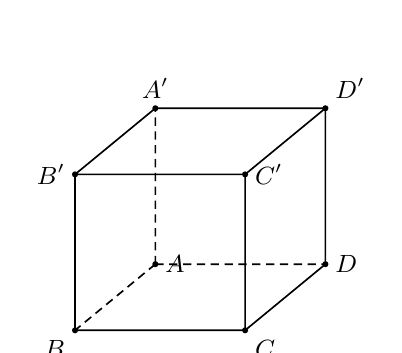
\begin{tikzpicture}[x=.60cm,y=.60cm,line width=.6pt,every node/.style={font=\small}]
 \coordinate (A) at (1.7,1.4); \coordinate (B) at (0,0);
 \coordinate (C) at (3.6,0); \coordinate (D) at (5.3,1.4);
 \coordinate (Ap) at (1.7,4.7); \coordinate (Bp) at (0,3.3);
 \coordinate (Cp) at (3.6,3.3); \coordinate (Dp) at (5.3,4.7);
 \draw[densely dashed] (A)--(B) (A)--(D) (A)--(Ap);
 \draw (B)--(C)--(D)--(Dp)--(Ap)--(Bp)--(B)
       (Bp)--(Cp)--(Dp) (Cp)--(C);
 \foreach \p in {A,B,C,D,Ap,Bp,Cp,Dp}{\fill (\p) circle (1.1pt);}
 \node[right] at (A) {$A$}; \node[below left] at (B) {$B$};
 \node[below right] at (C) {$C$}; \node[right] at (D) {$D$};
 \node[above] at (Ap) {$A'$}; \node[left] at (Bp) {$B'$};
 \node[right] at (Cp) {$C'$}; \node[above right] at (Dp) {$D'$};
\end{tikzpicture}\end{notebox}}
\newcommand{\cranefig}{%
\begin{notebox}\centering
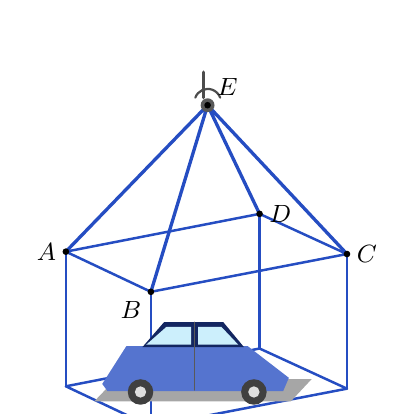
\begin{tikzpicture}[x=.60cm,y=.60cm,line join=round,line cap=round,every node/.style={font=\small}]
 \coordinate (E) at (0,6.15);
 \coordinate (A) at (-3,3.05); \coordinate (B) at (-1.20,2.20);
 \coordinate (C) at (2.95,3.00); \coordinate (D) at (1.10,3.85);
 \coordinate (Ab) at (-3,.20); \coordinate (Bb) at (-1.20,-.65);
 \coordinate (Cb) at (2.95,.15); \coordinate (Db) at (1.10,1.00);
 \draw[line width=1.2pt,grblue] (E)--(A) (E)--(B) (E)--(C) (E)--(D);
 \draw[grblue,line width=.9pt] (A)--(B)--(C)--(D)--cycle;
 \draw[grblue,line width=.9pt] (A)--(Ab) (B)--(Bb) (C)--(Cb) (D)--(Db);
 \draw[grblue,line width=.9pt] (Ab)--(Bb)--(Cb)--(Db)--cycle;
 \draw[very thick,gray!60!black] (-.08,6.85)--(-.08,6.31);
 \fill[gray!70!black] (E) circle (2.5pt);
 \draw[thick,gray!60!black] (-.26,6.31) arc[start angle=160,end angle=20,radius=.28];
 \fill[black!35] (-2.40,-.12)--(1.76,-.12)--(2.20,.35)--(-1.95,.35)--cycle;
 \fill[grblue!78] (-2.23,.25)--(-1.72,1.05)--(.85,1.05)--(1.72,.38)--(1.60,.10)--(-2.12,.10)--cycle;
 \fill[grblue!50!black] (-1.38,1.03)--(-.92,1.56)--(.33,1.56)--(.77,1.03)--cycle;
 \fill[cyan!20] (-1.30,1.08)--(-.87,1.46)--(-.35,1.46)--(-.35,1.08)--cycle;
 \fill[cyan!20] (-.20,1.08)--(-.20,1.46)--(.29,1.46)--(.65,1.08)--cycle;
 \draw[black!65,thin] (-.27,.12)--(-.27,1.56);
 \fill[black!75] (-1.42,.08) circle (.27) (.98,.08) circle (.27);
 \fill[gray!25] (-1.42,.08) circle (.12) (.98,.08) circle (.12);
 \foreach \p/\where in {E/above right,A/left,B/below left,C/right,D/right}
    {\fill (\p) circle (1.2pt);\node[\where] at (\p) {$\p$};}
\end{tikzpicture}\end{notebox}}

\begin{document}
\fontsize{11.5}{14}\selectfont
\examtitle{TDMXX20}{CƠ BẢN VỀ VECTƠ TRONG KHÔNG GIAN}
\partone{12}

\question[TDM21]{1} Cho hình hộp $ABCD.A'B'C'D'$. Hỏi đáp án nào sau đây cho nhận xét \textbf{sai}?
\twochoices{$\overrightarrow{AB}=\overrightarrow{C'D'}$.}{$\overrightarrow{AC}=\overrightarrow{A'C'}$.}
{$\overrightarrow{AA'}=\overrightarrow{CC'}$.}{$\overrightarrow{AD}=\overrightarrow{B'C'}$.}

\question[TDM21]{2} Cho hình hộp $ABCD.A'B'C'D'$. Nếu chỉ xét các vectơ có các điểm đầu và điểm cuối là các đỉnh của hình hộp đã cho thì có tất cả bao nhiêu vectơ mà tổng của nó với vectơ $\overrightarrow{AC}$ bằng vectơ-không?
\fourchoices{$4$.}{$1$.}{$3$.}{$2$.}

\question[TDM21]{3} Cho tứ diện $ABCD$ có $G$ là trọng tâm của tam giác $BCD$. Hệ thức đúng là
\twochoices{$\overrightarrow{AB}+\overrightarrow{AC}+\overrightarrow{AD}+3\overrightarrow{AG}=\vec{0}$.}
{$\overrightarrow{AB}+\overrightarrow{AC}+\overrightarrow{AD}=\overrightarrow{AG}$.}
{$\overrightarrow{AB}+\overrightarrow{AC}+\overrightarrow{AD}=3\overrightarrow{AG}$.}
{$\overrightarrow{GB}+\overrightarrow{GC}+\overrightarrow{GD}=3\overrightarrow{GA}$.}

\question[TDM21]{4} Cho bốn điểm $A,B,C,D$ bất kì trong không gian. Hệ thức \textbf{đúng} là
\twochoices{$\overrightarrow{AB}+\overrightarrow{CD}=\overrightarrow{AC}+\overrightarrow{DB}$.}
{$\overrightarrow{AB}+\overrightarrow{CD}=\overrightarrow{AD}+\overrightarrow{CB}$.}
{$\overrightarrow{AB}+\overrightarrow{CD}=\overrightarrow{AC}+\overrightarrow{BD}$.}
{$\overrightarrow{AB}+\overrightarrow{CD}=\overrightarrow{AD}+\overrightarrow{BC}$.}

\question[TDM21]{5} Cho hình hộp chữ nhật $ABCD.A'B'C'D'$ có các cạnh $AB=8$, $AD=6$, $AA'=10$. Đáp án cho nhận xét \textbf{sai} là
\twochoices{$\left|\overrightarrow{AB}\right|=8$.}
{$\left|\overrightarrow{AB}+\overrightarrow{AD}\right|=10$.}
{$\left|\overrightarrow{AB}+\overrightarrow{AD}+\overrightarrow{AA'}\right|=10\sqrt{2}$.}
{$\left|\overrightarrow{AB}+\overrightarrow{BD}+\overrightarrow{DA'}\right|=10\sqrt{2}$.}

\question[TDM21]{6} Cho hình hộp $ABCD.A'B'C'D'$. Đáp án cho nhận xét \textbf{sai} là
\twochoices{$\overrightarrow{AB}+\overrightarrow{BB'}+\overrightarrow{CD}=\overrightarrow{CC'}$.}
{$\overrightarrow{AB}+\overrightarrow{CD'}+\overrightarrow{D'D}=\vec{0}$.}
{$\overrightarrow{AB}+\overrightarrow{DA}+\overrightarrow{AA'}=\overrightarrow{AC'}$.}
{$\overrightarrow{BC}-\overrightarrow{CC'}-\overrightarrow{CD}=\overrightarrow{A'C}$.}

\question[TDM21]{7} Trong không gian, cho hai vectơ $\vec a,\vec b$ có $|\vec a|=4$, $|\vec b|=6$ và $\vec a\cdot\vec b=12\sqrt{2}$. Góc $(\vec a,\vec b)$ bằng
\fourchoices{$45^\circ$.}{$60^\circ$.}{$30^\circ$.}{$120^\circ$.}

\question[TDM31]{8} Cho hình lập phương $ABCD.A'B'C'D'$ có cạnh bằng $2$. Hãy tính $\overrightarrow{AC}\cdot\overrightarrow{BC'}$?
\cubefig
\fourchoices{$2\sqrt{2}$.}{$4\sqrt{2}$.}{$2\sqrt{3}$.}{$4$.}

\question[TDM32]{9} Cho hình lập phương $ABCD.A'B'C'D'$ có cạnh bằng $2$. Tích vô hướng của hai vectơ $\overrightarrow{AC'}$ và vectơ $\overrightarrow{B'D}$ bằng
\cubefig
\fourchoices{$2$.}{$4\sqrt{2}$.}{$-4$.}{$4$.}

\needspace{3\baselineskip}
\question[TDM31]{10} Trong không gian, cho hai vectơ $\vec a,\vec b$ có $|\vec a|=4$, $|\vec b|=2$ và $(\vec a,\vec b)=60^\circ$. Hãy tính giá trị của biểu thức $(\vec a+\vec b)\cdot(2\vec a-\vec b)$?
\fourchoices{$34$.}{$32$.}{$30$.}{$40$.}

\question[TDM32]{11} Cho tứ diện $ABCD$ có $\overrightarrow{AB}\cdot\overrightarrow{CD}+\overrightarrow{AC}\cdot\overrightarrow{DB}=12$. Hãy tính $\overrightarrow{AD}\cdot\overrightarrow{BC}$?
\fourchoices{$12$.}{$6$.}{$-12$.}{$-6$.}

\question[TDM32]{12} Cho tứ diện $ABCD$. Gọi $M,N$ lần lượt là trung điểm của $AB$ và $CD$. Đáp án cho nhận xét \textbf{sai} là
\twochoices{$\overrightarrow{MN}=\dfrac12(\overrightarrow{AD}+\overrightarrow{BC})$.}
{$\overrightarrow{MN}=\dfrac12(\overrightarrow{AC}+\overrightarrow{BD})$.}
{$\overrightarrow{AD}+\overrightarrow{BC}=\overrightarrow{AC}+\overrightarrow{BD}$.}
{$\overrightarrow{MN}=\dfrac12(\overrightarrow{AB}+\overrightarrow{CD})$.}

\parttwo{13}{16}
\question[TDM31]{13} Cho hai vectơ $\vec a,\vec b$ và các số thực $h,k$. Mệnh đề nào sau đây là \textbf{đúng hay sai}?
\tfbox{$k(\vec a+\vec b)=k\vec a+k\vec b$.}
{$(h+k)\vec a=h\vec a+\vec a k$.}
{$k\vec a-k\vec b=k(\vec a-\vec b)$.}
{$h\vec a+k\vec a=\vec0\Leftrightarrow h+k=0$.}

\question[TDM32]{14} Cho hình lập phương $ABCD.A'B'C'D'$. Mệnh đề nào sau đây là \textbf{đúng hay sai}?
\tfbox{Góc của hai vectơ $\overrightarrow{AD}$ và $\overrightarrow{B'C'}$ bằng $0^\circ$.}
{Góc giữa hai vectơ $\overrightarrow{AC}$ và $\overrightarrow{C'A'}$ bằng $0^\circ$.}
{$(\overrightarrow{AC},\overrightarrow{A'B})=60^\circ$.}
{$\cos(\overrightarrow{AC'},\overrightarrow{CD})=\dfrac{1}{\sqrt3}$.}

\question[TDM32]{15} Cho ba vectơ $\vec a,\vec b,\vec c$ trong không gian. Mệnh đề nào sau đây là \textbf{đúng hay sai}?
\tfbox{$\vec a\cdot\vec b=\vec b\cdot\vec a$.}
{$\vec a\cdot(\vec b-\vec c)=\vec a\cdot\vec b-\vec a\cdot\vec c$.}
{$(2\vec a-3\vec b)^2=2\vec a^{\,2}+3\vec b^{\,2}-12\vec a\cdot\vec b$.}
{$(\vec a\cdot\vec b)\vec c=(\vec b\cdot\vec a)\vec a=(\vec c\cdot\vec a)\vec b$.}

\question[TDM32]{16} Cho hai vectơ $\vec a,\vec b\ne\vec0$, số thực $k\in\mathbb R$, hai điểm $A$ và $B$ phân biệt. Mệnh đề nào sau đây là \textbf{đúng hay sai}?
\tfbox{$(\vec a,\vec b)=(\vec b,\vec a)$.}
{Với mọi $k\in\mathbb R$ ta luôn có $(k\vec a,\vec b)=(\vec a,\vec b)$.}
{$(\vec a,\overrightarrow{AB})=180^\circ-(\vec a,\overrightarrow{BA})$.}
{$(\vec a,\overrightarrow{AB})+(\overrightarrow{AB},\vec b)=(\vec a,\vec b)$.}

\partthree{17}{22}
\question[TDM31]{17} Cho tứ diện $ABCD$ có $AB=6$, $CD=8$ và $\overrightarrow{AB}\cdot\overrightarrow{CD}=-30$. Hãy xác định góc giữa hai đường thẳng $AB$ và $CD$ theo đơn vị độ? (Làm tròn kết quả đến hàng phần mười)
\shortanswer

\question[TDM32]{18} Cho một toà nhà gồm có $40$ tầng. Chiều cao của $20$ tầng đầu tiên là $76$ mét chia đều cho mỗi tầng, $20$ tầng tiếp theo có chiều cao mỗi tầng là bằng nhau. Một chiếc thang máy khi di chuyển từ tầng $15$ lên tầng $23$ có vectơ biểu diễn độ dịch chuyển là $\vec a$, khi di chuyển từ tầng $23$ lên tầng $33$ có vectơ biểu diễn độ dịch chuyển là $\vec b$. Biết rằng $\vec a=\vec b$. Hãy xác định chiều cao của tầng thứ $30$ theo đơn vị mét? (Làm tròn kết quả đến hàng phần trăm)
\shortanswer

\question[TDM32]{19} Một chiếc ôtô được đặt trên mặt đáy dưới của một khung sắt có dạng hình hộp chữ nhật với đáy trên là hình chữ nhật $ABCD$, có mặt phẳng $(ABCD)$ song song với mặt phẳng nằm ngang. Khung sắt được buộc vào móc $E$ của chiếc cần cẩu sao cho các đoạn dây cáp $EA,EB,EC,ED$ có độ dài bằng nhau và cùng tạo với mặt phẳng nằm ngang một góc bằng $60^\circ$. Chiếc cần cẩu kéo khung sắt lên theo phương thẳng đứng. Biết trọng lượng của khung sắt bằng $4000\,\mathrm{N}$ và độ lớn lực căng của mỗi dây cáp là $3800\,\mathrm{N}$. Hãy xác định trọng lượng của chiếc ôtô theo đơn vị Niutơn? (Làm tròn kết quả đến hàng đơn vị)
\cranefig
\shortanswer

\question[TDM42]{20} Cho tứ diện $ABCD$ có $AD=8\,\mathrm{cm}$, $BC=10\,\mathrm{cm}$ và $(\overrightarrow{AD},\overrightarrow{CB})=60^\circ$. Gọi $M,N$ lần lượt là trung điểm của các cạnh $AB,CD$. Hãy xác định độ dài đoạn $MN$ theo đơn vị cm? (Kết quả được làm tròn và lấy hai chữ số sau dấu phẩy)
\shortanswer

\question[TDM42]{21} Cho hình chóp $S.ABCD$ có đáy là hình vuông cạnh bằng $6\,\mathrm{cm}$, có $SA\perp BC$, tam giác $SAB$ đều. Gọi $M,N$ là hai điểm thoả mãn $\overrightarrow{SM}=2\overrightarrow{MA}$, $\overrightarrow{CN}+2\overrightarrow{BN}=\vec0$. Hãy xác định độ dài đoạn $MN$ theo đơn vị cm? (Kết quả được làm tròn và lấy hai chữ số sau dấu phẩy)
\shortanswer

\question[TDM42]{22} Trong không gian cho hai vectơ $\vec a,\vec b$ thoả mãn $|2\vec a+\vec b|=12$ và $|\vec a-3\vec b|=3\sqrt{11}$. Hãy xác định giá trị của biểu thức $2\vec a^{\,2}+3\vec b^{\,2}$? (Kết quả được làm tròn đến hàng đơn vị)
\shortanswer
\finishExam

% Nguon: DE TDMXX20_DTL_CO BAN VE VECTO TRONG KHONG GIAN_PB1.pdf (4 trang).
% Ban LaTeX: BTVN_B7.tex; hinh minh hoa duoc ve lai bang TikZ.
\end{document}
